%!TEX root = tesis.tex


\chapter{Un \ssolver paralelo y distribuido }
\label{ssolver-pardist}

La implementación de nuestra herramienta como un sistema distribuido persigue
el objetivo fundamental de mejorar el tiempo de ejecución ya sea decrementando
el tiempo necesario para resolver un problema determinado, o transformando un
problema previamente irresoluble (en tiempo razonable) en resoluble. Para ello
el sistema debe ser \textbf{escalable} en tanto que debe tener la capacidad de
sacar provecho de la incorporación una mayor cantidad de \hard a la infraestructura
utilizada en la resolución del problema. Por otro
lado, el uso de este \hard debe ser \textbf{eficiente} en el sentido de que la
utilización de mayor cantidad de \hard debe resultar en un mejora de la
performance del sistema (en nuestro caso entendida como se describió
previamente).

\begin{wrapfigure}{R}{0.4\textwidth}
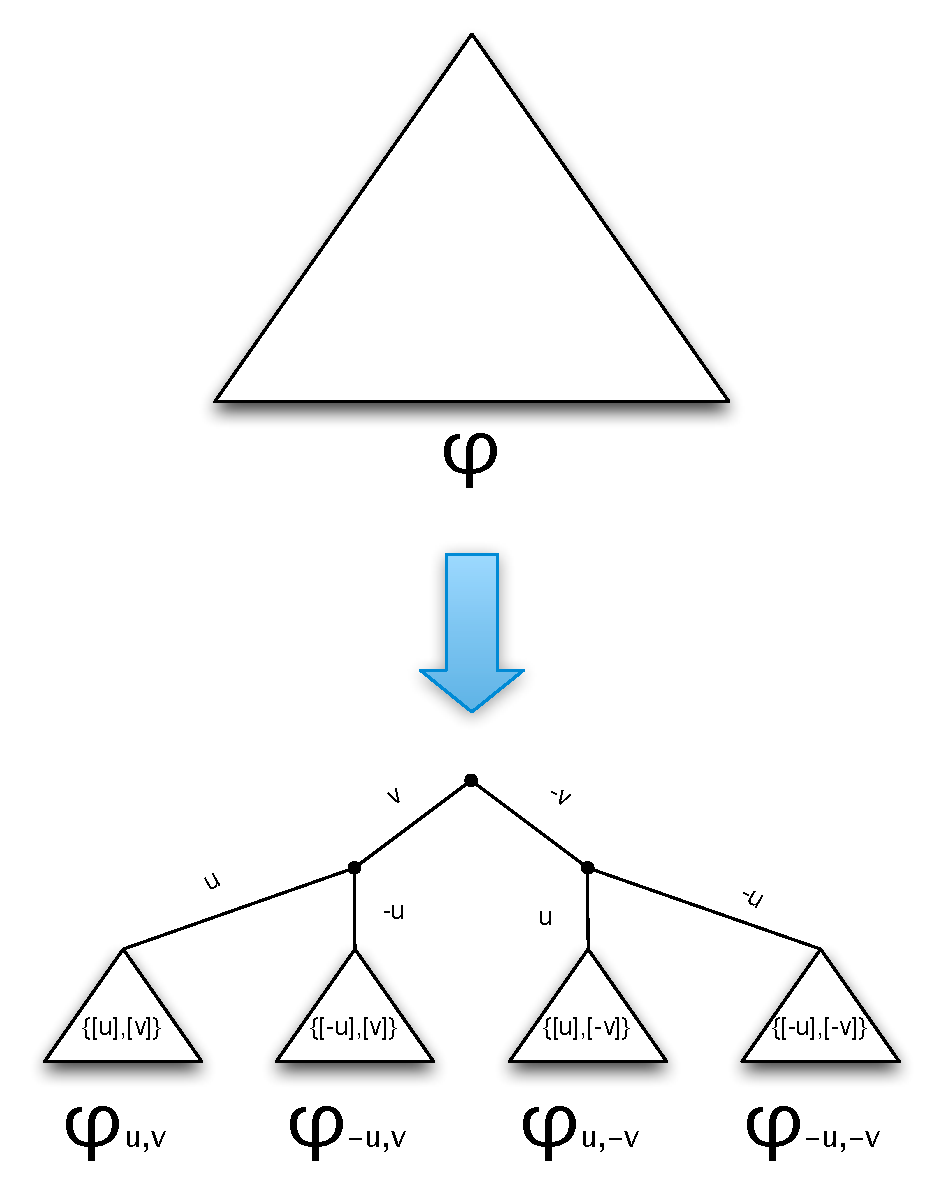
\includegraphics[scale=0.4]{graphs/split por guiding path}
\caption{Esquema de partición por \gp}
\label{fig:guidingpaths}
\end{wrapfigure}

Con estos dos objetivos en mente desarrollamos una \ssolver distribuido basado
en la idea de \gp y orientado a que su utilización sea en \clusters de computadoras. La idea de \gp se
basa en la observación de que, en el peor caso, todas las posibles valuaciones
de una fórmula proposicional $\varphi$ deben ser evaluadas. Una vez que una
valuación que satisface a una fórmula es encontrada, el procedimiento de
\ssolving puede darse por finalizado\footnote{Existe otra variante en la que, además
de determinar si una fórmula es \sat o \unsat, interesa enumerar todos los
posibles modelos de dicha fórmula. En este escenario el procedimiento de
\ssolving no puede ser detenido una vez que se encuentra una valuación sino
que el mismo debe continuar hasta agotar todas las posibles valuaciones que
satisfacen a la fórmula en cuestión.}. Por el contrario, si la fórmula es
\unsat, la única alternativa para poder asegurarlo es agotar todas las
posibles valuaciones y determinar que ninguna de ellas satisface a la fórmula
en cuestión. Por lo tanto, una forma de dividir el problema es tomar una
variable $v$ y construir los dos subproblemas $\varphi_{v \leftarrow 0}$ y
$\varphi_{v \leftarrow 1}$ que se derivan de las dos posibles asignaciones de
valores de verdad a dicha variable. Una vez hecho esto, determinar que el
problema original $\varphi$ es \unsat se reduce a determinar que tanto
$\varphi_{v \leftarrow 0}$ como $\varphi_{v \leftarrow 1}$ son \unsat. Por el
contrario, determinar que el problema es \sat reduciría a establecer que
$\varphi_{v \leftarrow 0}$ es \sat o bien que $\varphi_{v \leftarrow 1}$ lo
es. Ahora, $\varphi_{v \leftarrow 0}$ y $\varphi_{v \leftarrow 1}$ pueden ser
considerados como dos problemas independientes y volver a aplicar la misma
idea recursivamente. Naturalmente este proceso puede realizarse seleccionando
más de una variable en cada paso. Al seleccionar $n$ variables obtendremos
entonces $2^n$ subproblemas. Llamaremos \emph{levantar variables} al proceso
de dividir un problema $\varphi$ en los $2^n$ subproblemas que resultan de
aplicar todas las posibles valuaciones sobre el conjunto de $n$ variables
levantadas. Se desprende de esto que una de las tareas que debe poder realizar
la herramienta es la de dividir un problema en los subproblemas que derivan de 
adoptar todos los posible \gp para un conjunto de variables.

% El objetivo principal de todo sistema distribuido es que el mismo sea
% \textbf{escalable}. Si bien la escalabilidad puede ser entendidad en
% diferentes sentidos, nos interesa en particular que el sistema haga posible la
% utilización de mayor cantida de \hard para resolver el problema (en nuestro
% caso un problema \sat) y que esa utilización de mayor poder de cómputo reporte
% ganancias en términos de tiempo (percibido) invertido en resolver un
% determinado problema o bien en términos de empujar la frontera de lo
% resoluble.

%La escalabilidad como gran objetivo rector en el desarrollo de nuestra
%herramienta introduce una serie de desafíos, a saber:
%\begin{itemize}
%	\item Almacenamiento distribuido.
%	\item Simetría de capacidades en los nodos de trabajo (\ws).
%	\item Minimización de la utilización de la red de comunicaciones.
%\end{itemize}


\section{Objetivos de diseño y desafíos asociados}

\subsection{Aspectos básicos de escalabilidad}

En primer término consideraremos los desafíos asociados con ciertos aspectos
básicos que, de no ser adecuadamente manejados, podrían atentar de modo flagrante
contra la escalabilidad de la herramienta.

\subsubsection{Almacenamiento distribuido}

La necesidad de que el almacenamiento de problemas pendientes de resolución se
encuentre distribuido se debe a un doble aspecto. Por un lado, la cantidad de
subproblemas producidos puede ser muy grande. Por lo tanto no es razonable
requerir que la cantidad de espacio necesario para almacenar todas las tareas
pendientes de resolución se encuentre disponible en una misma ubicación.

Aún si fuera posible contar con la cantidad de espacio necesaria para almacenar
todos los subproblemas en una ubicación centralizada, surge un segundo problema
que presentaría este enfoque: el de la contención de acceso a la información asociada a un problema. 
Si pretendemos que el almacenamiento no se vuelva un cuello de botella, es vital
distribuir las tareas pendientes de modo que cuando los \ws requieran nuevas
tareas para resolver, los múltiples pedidos no recaigan siempre sobre un mismo equipo.


\subsubsection{Simetría en las capacidades de los \ws}

El requisito de que los nodos de trabajo (\ws) sean simétricos también se desprende
de la necesidad de eliminar los potenciales cuellos de botella. La simetría, entendida en su
máxima expresión como la posibilidad de que todas las unidades de
procesamiento puedan realizar todas las funciones necesarias, provee la
capacidad de distribuir la carga de trabajo de la manera más conveniente en
cada momento.

Esto no podría lograrse si los nodos de trabajo tuvieran
funciones específicas, ya que podría darse el caso de tener nodos ociosos
por falta de trabajo pendiente de la clase de trabajo que esos nodos realizan, 
a la vez que otros nodos se encuentran sobrecargados. Esta situación podría empeorar
seriamente a medida que la cantidad de nodos aumenta.

En nuestro caso particular, el requisito de simetría se traduce en que
todos los \ws deben poseer las capacidades de: \begin{inparaenum}[a)] \item analizar un
subproblema hasta lograr obtener un veredicto (consumir), \item
dividir un subproblema demasiado difícil en nuevos subproblemas (producir) y \item almacenar,
solicitar y transferir subproblemas (distribuir). \end{inparaenum}


\subsubsection{Movilidad de tareas pendientes}

El triple rol de productor, consumidor y distribuidor asignado a los \ws
transforma la migración de tareas en un desafío en tanto que un \w puede
estar --y generalmente lo estará-- ocupado analizando un
subproblema cuando otro \w le solicite algún subproblema
pendiente que se encuentre en su poder.

Es claro que, ante esta situación, no sería aceptable que el \w que está
esperando una tarea se vea obligado a esperar hasta que aquel que la generó
deje de \solvear para poder acceder a la misma. Esto da origen a un requerimiento
de asincronicidad entre \emph{solving} y \emph{serving}.

Sin embargo, tampoco sería aceptable que el impacto de servir tareas bajo demanda vaya en
detrimento del análisis, que es, al fin y al cabo, el verdadero objetivo del \w.
De aquí surgen un requerimiento de sincronicidad (por ejemplo: encolar los pedidos de
tareas pendientes y atender sólo una cantidad limitada a la vez) y otro de balanceo
de carga (por ejemplo: evitar que la capacidad de almacenamiento de un \w llegue a
saturarse transfiriendo preventivamente tareas a otros \ws).

En resumen, lograr ortogonalidad entre análisis y migración de tareas es
importante para lograr escalabilidad, y sienta las bases para el desarrollo de mecanismos
avanzados de balanceo automático de carga.



\subsection{Aspectos de automatización e interactividad}

La automatización de la operatoria es un requerimiento crucial. Desde el punto
de vista del usuario, es fundamental que la herramienta sea capaz de llevar a
cabo su objetivo --demostrar la propiedad o exhibir un contraejemplo-- sin requerir
supervisión alguna ni depender de complejas parametrizaciones que requieran
numerosos experimentos para ser halladas.

Sin embargo, generar una estrategia automática que proporcione buenos resultados
en la ejecución de un amplio espectro de problemas es sumamente difícil. Desde el
punto de vista del experto que necesita diseñar, implementar, evaluar, depurar y
mejorar una estrategia no supervisada, es importante contar con alguna
interfaz interactiva que posibilite la inyección de comandos arbitrarios que permitan 
la modificación del comportamiento de la herramienta en tiempo de ejecución.

La necesidad de atender estos requerimientos encontrados motivó la adopción de
un enfoque en el que la maquinaria de cómputo distribuido (i.e. la comunidad de \ws) no posee inteligencia
propia, sino que se limita a proveer una serie de funcionalidades básicas que
pueden ser invocadas remotamente, ofreciendo un alto grado de generalidad. La
operación del sistema se lleva a cabo desde un tablero de control que permite
explorar manualmente trazas de ejecución arbitrarias. Sobre esto se monta
luego la automatización; en primer término la de aspectos reiterativos de rutina (i.e. carga de tareas al momento de la liberación de la unidad de cómputo, etc.),
y finalmente la que implementa la toma inteligente de decisiones estratégicas (i.e. cuándo es conveniente partir un problema en subproblemas, etc.).

De lo antedicho surgen tres desafíos concretos. En primer lugar, el de lograr una
arquitectura adecuada para ser totalmente controlable por un operador remoto humano.
En segundo lugar, el de diseñar las interfaces de modo tal que provean una base adecuada
para automatizar, tanto parcial como totalmente, dicho control. Y finalmente el de
diseñar e implementar la estrategia automática propiamente dicha.


\subsection{Otros aspectos de calidad}

%Además de los as de escalabilidad, surgen también los desafíos
%relacionados con la eficiencia o la performance de la herramienta. Entre ellos
%los más destacados son:
%
%\begin{itemize}
%	\item Movilidad de tareas.
%	\item Crecimiento a la par de los \ssolvers secuenciales.
%	\item No hacer burradas \todo{Revisar toda esta itemización. No me convence....}
%\end{itemize}

\subsubsection{Modularidad del componente \ssolver de los \ws}

Otro de los objetivos que perseguimos a la hora de diseñar nuestra herramienta
fue que la misma pudiera utilizar un \ssolver \ots para la resolución local de
un subproblema concentrando las tareas vinculadas al desarrollo del \ssolver en 
los aspectos de orquestación del cómputo distribuido. Esto nos permite aprovechar 
los numerosos avances logrados por
la comunidad en el área de investigación en \ssolving secuencial en los últimos
años, y a la vez nos permite, a futuro, evolucionar a la par de los \ssolvers
secuenciales, capitalizando sus nuevos logros a bajo costo y mitigando el
riesgo de que la herramienta devenga obsoleta ante un nuevo avance en dicho
campo de estudio.

\subsubsection{Mantenibilidad y modificabilidad}

El último objetivo que perseguimos durante el desarrollo de nuestra
herramienta fue que la misma presentara facilidad para ser modificada sin que
esto impactara negativamente en la \emph{performance}. Este objetivo, entre
otras cosas, determinó la elección de las tecnologías a utilizar para su
desarrollo. Por lo tanto, se utilizó el lenguaje de programación \Python para
el desarrollo de toda la herramienta con excepción de las secciones destinadas al cómputo
intensivo.

Al utilizar un \ssolver \ots no fue necesario elegir un lenguaje
para su desarrollo. En la implementación actual de la herramienta utilizamos
el \ssolver \minisatdosveinte que está desarrollado en el lenguaje \cpp. Para
ello se desarrolló un \emph{wrapper} que permite utilizar \minisat desde un
entorno \Python, obteniendo todos los beneficios de un lenguaje de programación
dinámico sin pérdida de eficiencia en los algoritmos vinculados al cómputo intensivo.

Para el intercambio de mensajes entre los \ws se utilizó el
estándar \mpi a través de la biblioteca \texttt{mpi4py}\cite{mpi4py}.


% \begin{itemize}
% 	\item Escalable
% 	\item Uso de SAT Solver off-the-shelf
% 	\item Multiplataforma
% 	\item Tablero de control
% \end{itemize}

\section{Arquitectura}

La \fig\ref{fig:arquitectura} muestra la arquitectura de la herramienta. En
la misma se distinguen claramente dos componentes: el \bend que ejecuta sobre
un \cluster de computadoras y el \fend que ejecuta en un equipo que se
encuentra posiblemente fuera del centro de cómputos.

\begin{wrapfigure}{R}{0.45\textwidth}
\fbox{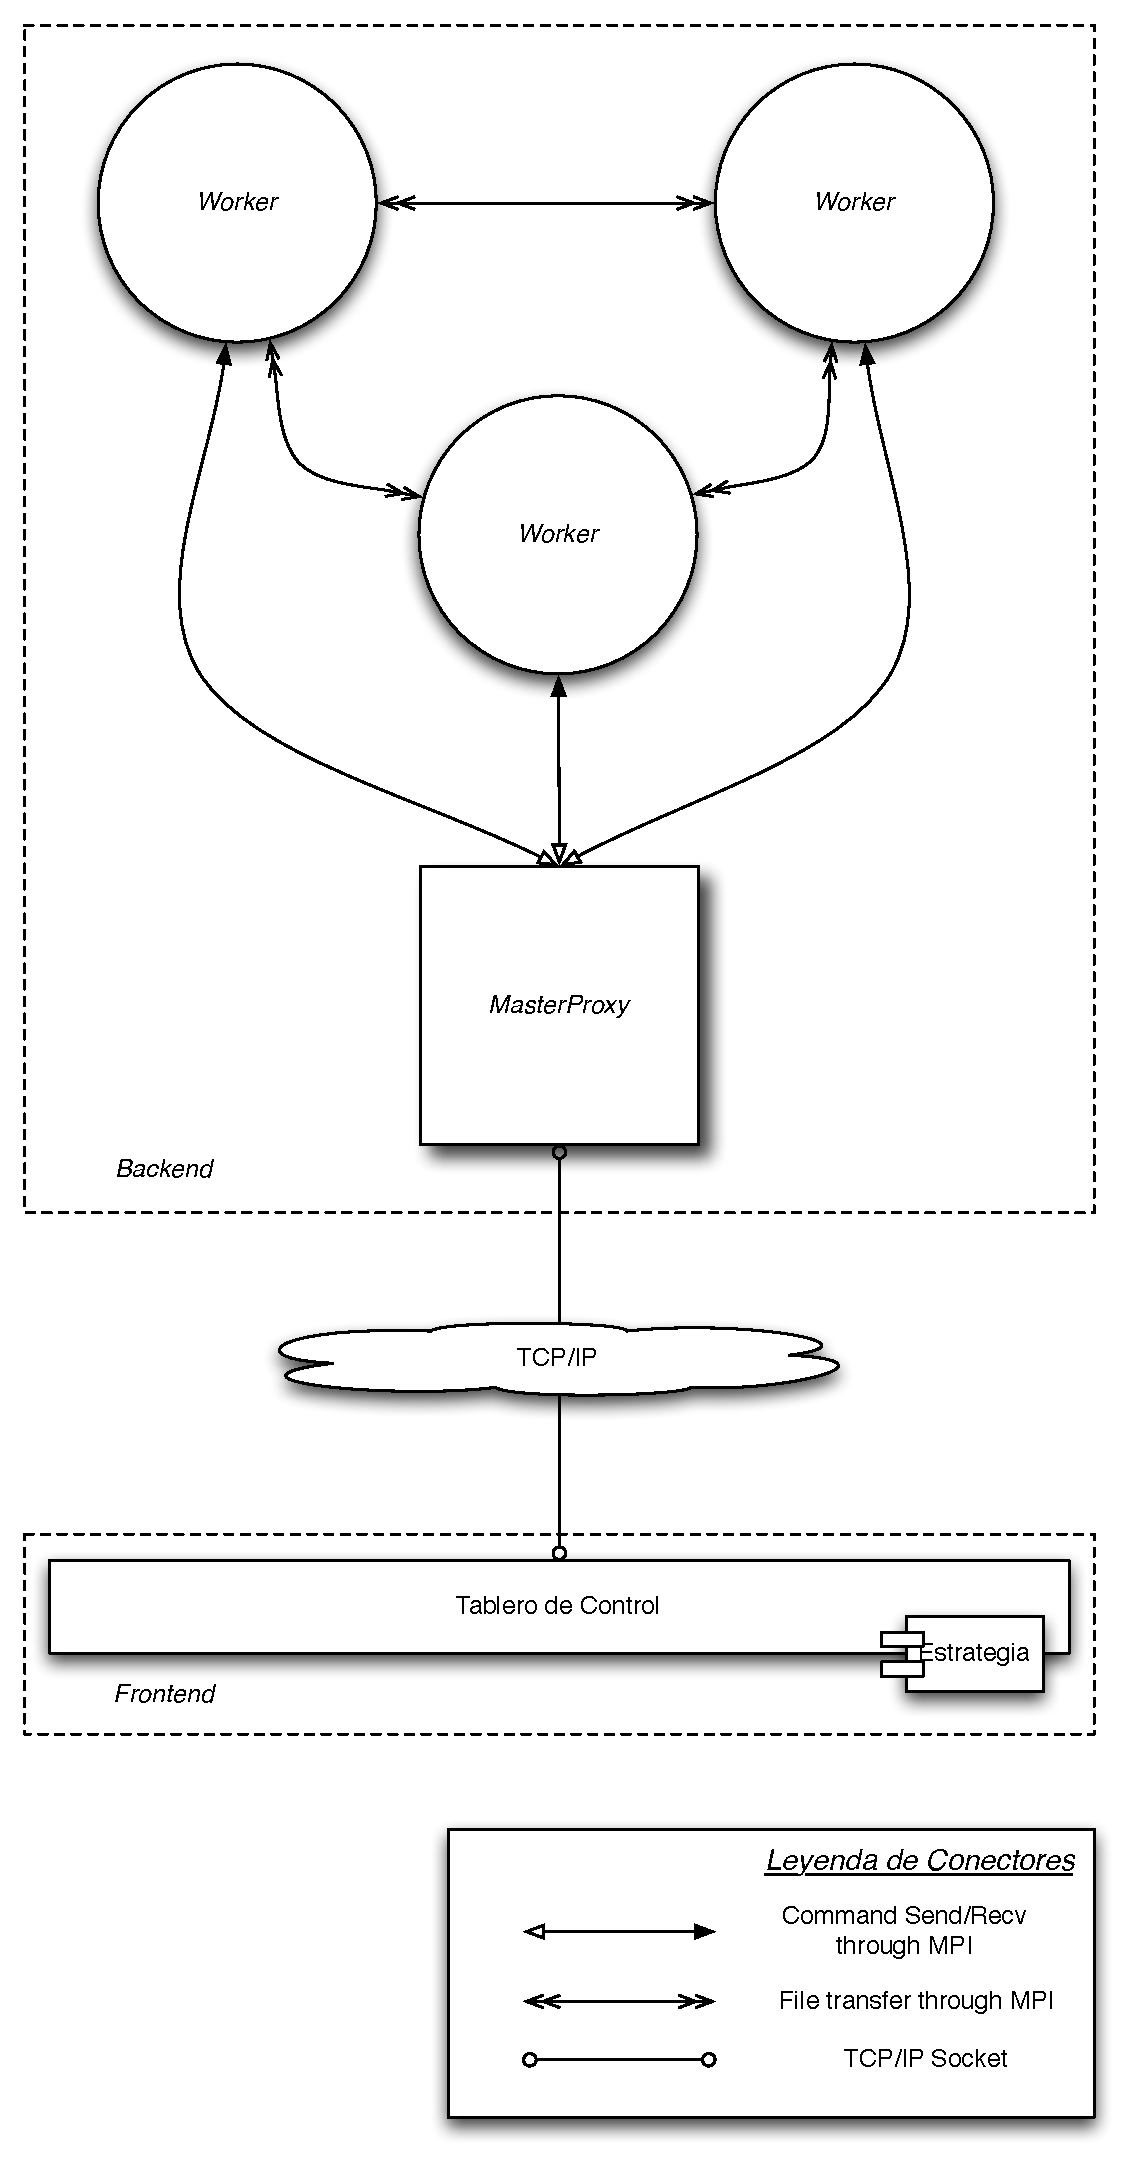
\includegraphics[scale=0.3]{graphs/paralloy architecture}}
\caption{Diagrama de componentes y conectores del \ssolver distribuido}
\label{fig:arquitectura}
\end{wrapfigure}

\subsection{\bend}
\label{sec:backend}

En el \bend se puede observar que existen dos clases distintas de elementos.
Por un lado tenemos un proceso llamado \master que es el encargado de manejar
la comunicación de órdenes desde el \fend hacia los \ws y de reenviar las
respuestas correspondientes desde los \ws hacia el \fend.

En segunda instancia encontramos otro de tipo de procesos, los \ws. Los \ws
son los encargados de relizar el cómputo (\ssolving) y la división de un
problema en nuevos subproblemas. Asimismo son quienes almacenan las tareas
pendientes de ejecución y por lo tanto deben proveer acceso a dicho
almacenamiento a los demás \ws.

Es importante destacar que si bien el \bend presenta una arquitectura
\masterslave, el \master en este caso no toma ninguna decisión sino que
simplemente actúa como intercambiador de mensajes entre el ambiente externo
(el \fend) y el ambiente interno.

\begin{figure}[h!]
\centering
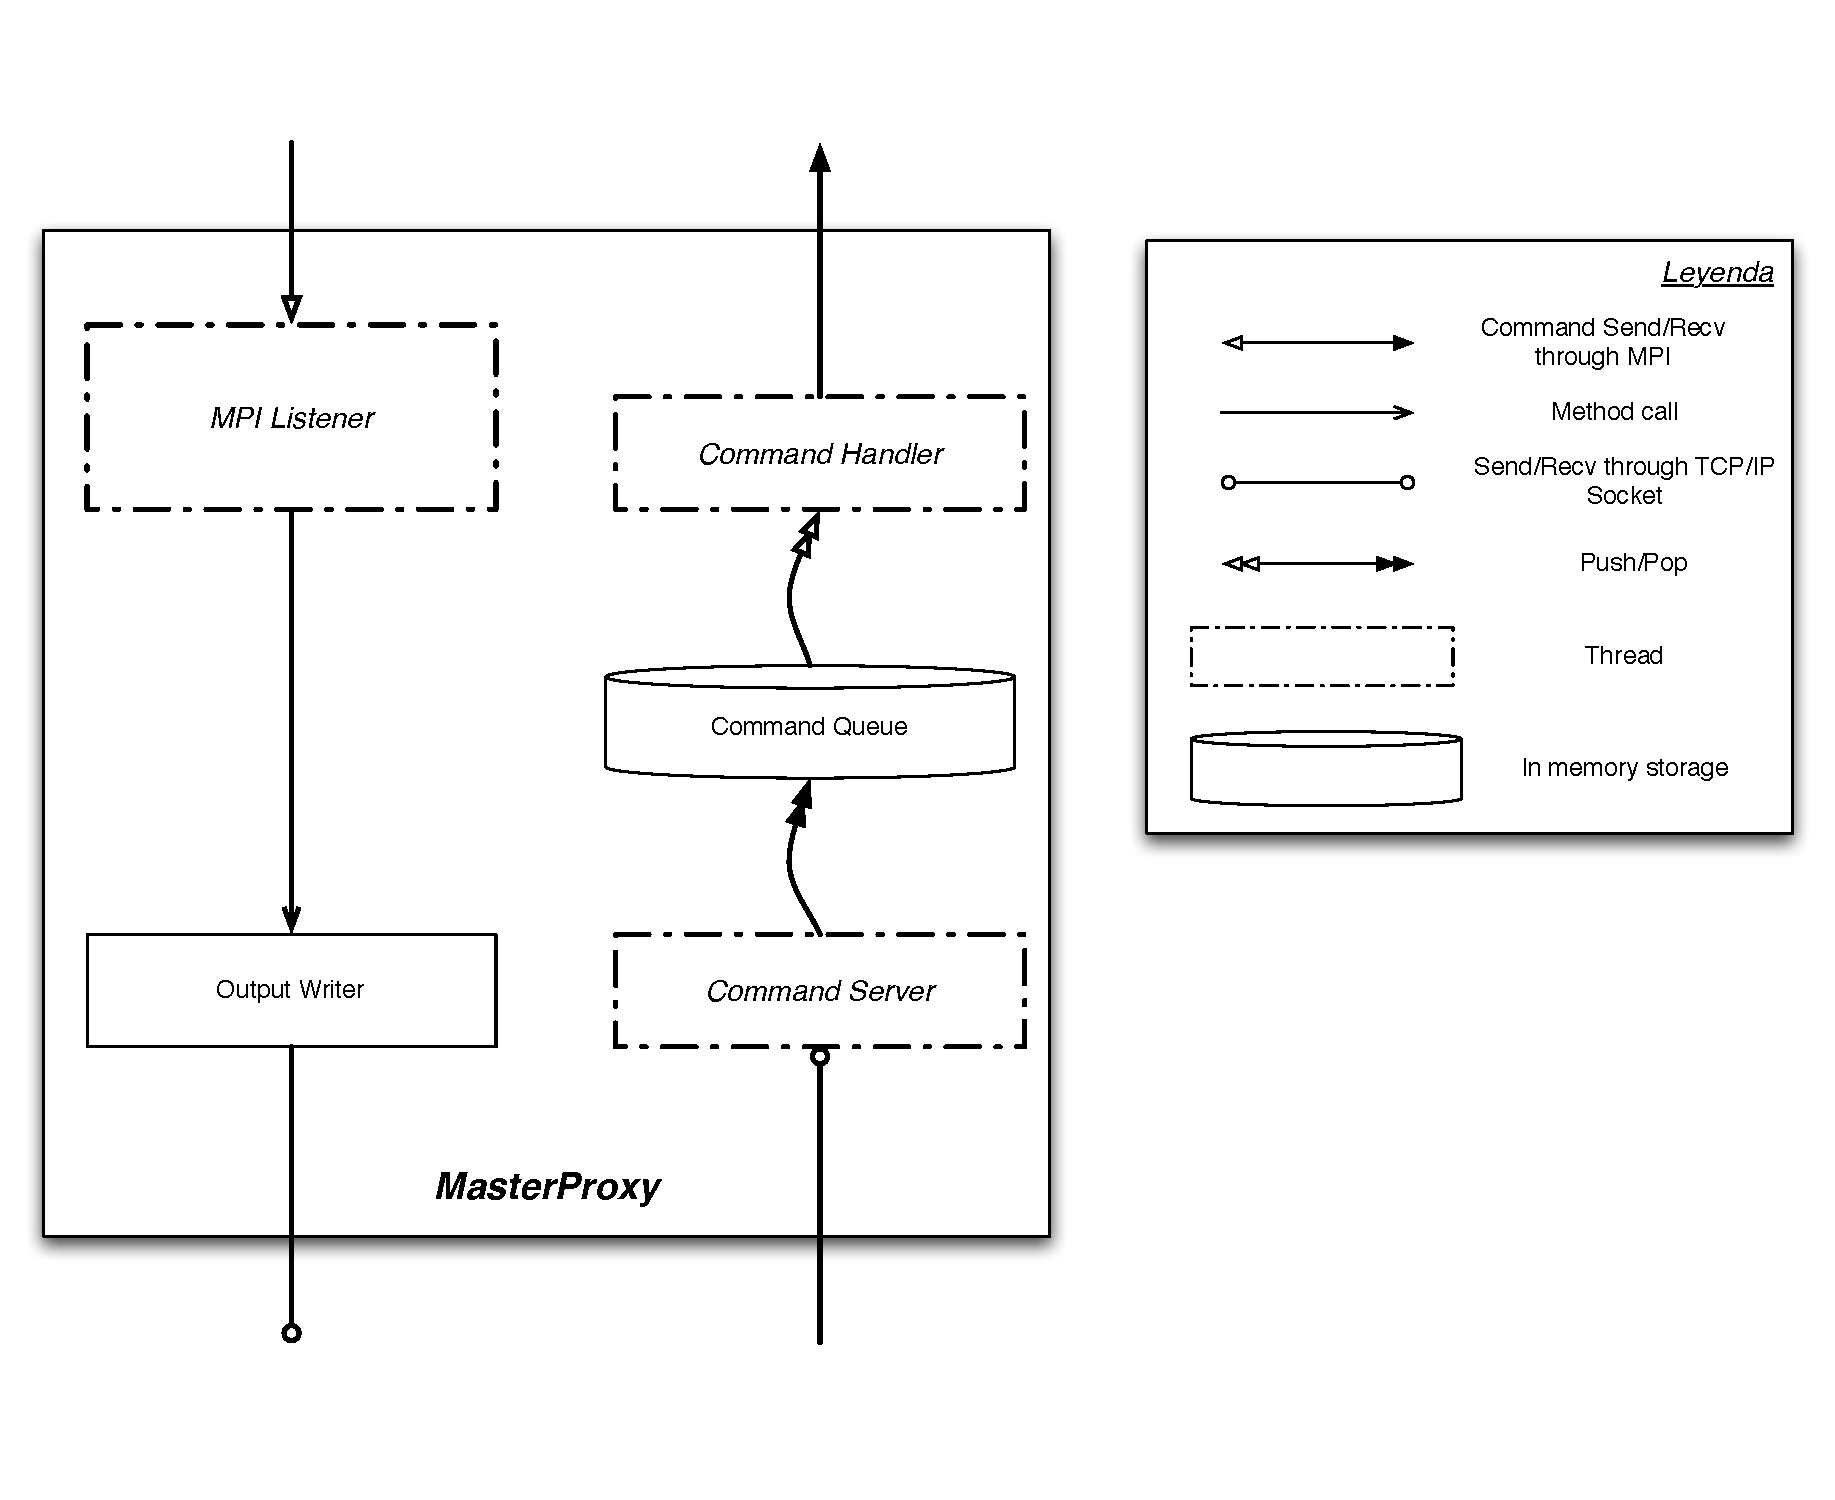
\includegraphics[scale=0.4]{graphs/master proxy detail}
\caption{Detalle de arquitectura del componente \master}
\label{fig:masterproxydetail}
\end{figure}

La \fig\ref{fig:masterproxydetail} detalla la arquitectura del \master. En el
diagrama se puede observar que el \datapath de entrada (\fend hacia \bend) y
el de salida (\bend hacia \fend) son independientes. Esto es una consecuencia
directa que se desprende de la ausencia de inteligencia en el \master. Esto
implica que no es necesario mantener el estado del sistema ya que en este
componente no se toman decisiones. La ausencia de estado hace que el proceso
\master consuma un mínimo de recursos, tanto de cómputo como de almacemiento.

La intervención de dos \threads distintos en el \datapath de entrada
proporciona un alto nivel de respuesta ya que permite que algunos comandos
sean implementados internamente mediante comunicación sincrónica a través de
\mpi sin que esto implique una pausa en el procesamiento del flujo de datos de
entrada desde el \fend hacia el \bend. La comunicación sincrónica permite
simplificar algunos comandos como el envío del problema original hacia todos
los \ws. Al mismo tiempo se mantiene el orden entre los comandos enviados
desde el \fend lo cual también contribuye a la simplificación del modelo de
cómputo a pesar de tratarse de un sistema distribuido.

\begin{figure}[h!]
\centering
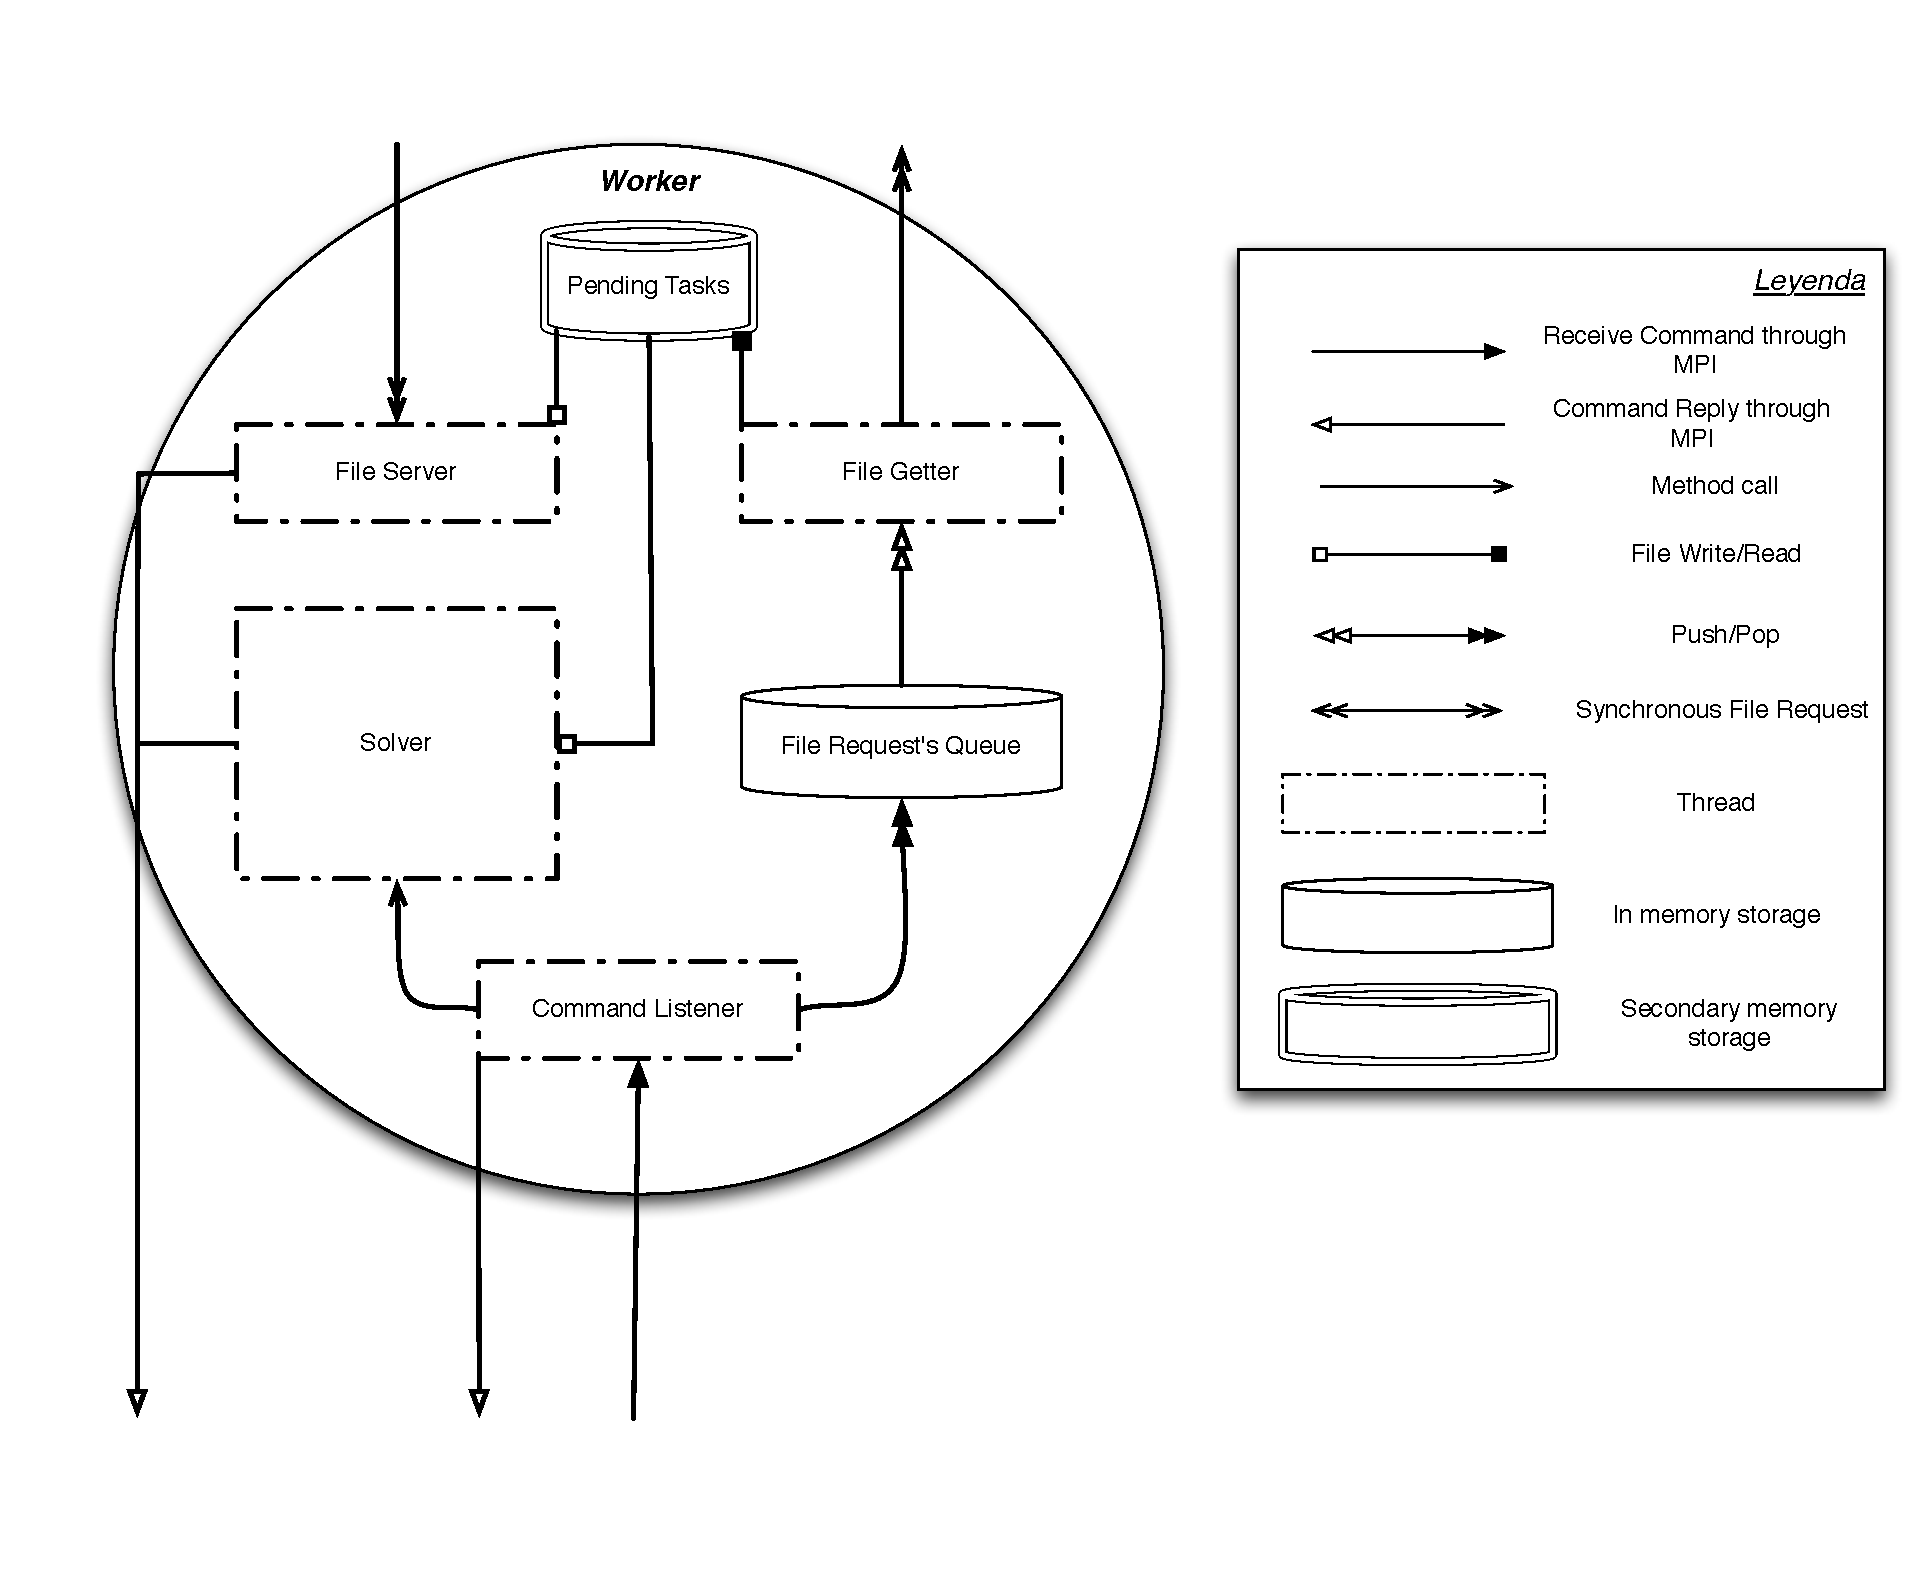
\includegraphics[scale=0.4]{graphs/worker detail}
\caption{Detalle de arquitectura del componente \w}
\label{fig:workerdetail}
\end{figure}

La \fig\ref{fig:workerdetail} muestra el detalle de diseño del componente
\w. Como se puede observar, las funciones de \solving, comunicación y
transferencia de archivos se implementaron en \threads separados. Dado que la
función de \solving utiliza principalmente tiempo de \cpu, mientras que el
resto de las funciones consumen principalmente tiempo de \io, la separación de
éstas en distintos \threads permite la ejecución concurrente de estas
tareas sin que esta característica impacte negativamente en el desempeño del
\ssolver. A la vez, esta característica permite satisfacer el objetivo de
movilidad de las tareas, aún cuando el \w se encuentre ocupado \solveando.

Interesa destacar también que la estrategia de partición de un problema
se encuentran implementadas en los \ws. Si
bien este diseño es contrario a la idea general basado en la existencia de un \emph{tablero de control}
consideramos que el nivel de granularidad necesario para poder controlar
remotamente la realización de estas dos tareas era demasiado alto y atentaba
contra la usabilidad de la herramienta. Asimismo, la herramienta es capaz de
poseer diversas estrategias implementadas
de modo que el usuario puede seleccionar aquella que le resulte más apropiada (y sus
parámetros en caso que corresponda) desde el \fend.

Por último, corresponde mencionar a qué nos referimos en concreto cuando
hablamos de \emph{tarea}. El término \emph{tarea} fue mencionado en varias
ocasiones a lo largo de la explicación. Si bien conceptualmente una tarea
podría ser simplemente una fórmula $\varphi$ en \cnf, en la práctica esto
podría producir un \emph{overhead} en la transferencia demasiado grande ya
que, por ejemplo al partir un problema levantando $n$ variables podríamos
generar $2^n$ subproblemas, cada uno de los cuales estaría representado
esencialmente por la misma fórmula $\varphi$ más las cláusulas unitarias
que determinan el \gp al que cada subproblema corresponde. Esta situación se repite innumerables veces a lo
largo de la ejecución de la herramienta para resolver un problema. Es por esto
que optamos, como modo de funcionamiento, por enviar la fórmula \cnf del problema original a
todos los \ws al comienzo de una ejecución de la herramienta de modo que luego
un subproblema esté representado sólo por el \gp identificado por las cláusulas unitarias necesarias para
forzar las decisiones correspondientes a ese subproblema. Esto hace que las
tareas pendientes de resolución sean mucho más económicas de manipular. 

Incluso pensando a futuro y considerando la posibilidad de implementar estrategias de
aprendizaje es necesario que, como parte de una tarea, se puedan transferir
también las cláusulas aprendidas que deban ser consideradas a los efectos de resolver esa tarea. Inclusive es
posible que en un futuro una tarea no represente únicamente un subproblema que
aún se debe intentar \solvear, sino que podría también incluir otro tipo de
actividades, como la partición de un problema. Esto último nos motivó a optar
por un concepto de tarea genérico donde una tarea no es más que un paquete de
archivos que el \w sabrá interpretar apropiadamente. En la implementación
actual las tareas son exclusivamente un subproblema pendiente de ser atacado y
se representan como un paquete con un archivo que incluye las cláusulas
unitarias que deben adicionarse al \cnf original para construir el subproblema
correspondiente más dos archivos que pueden o no contener información. Estos
últimos transportan la información de cláusulas aprendidas que deben ser
incorporados al intento de \solving del subproblema en cuestión.

\subsection{\fend}

\begin{figure}[h!]
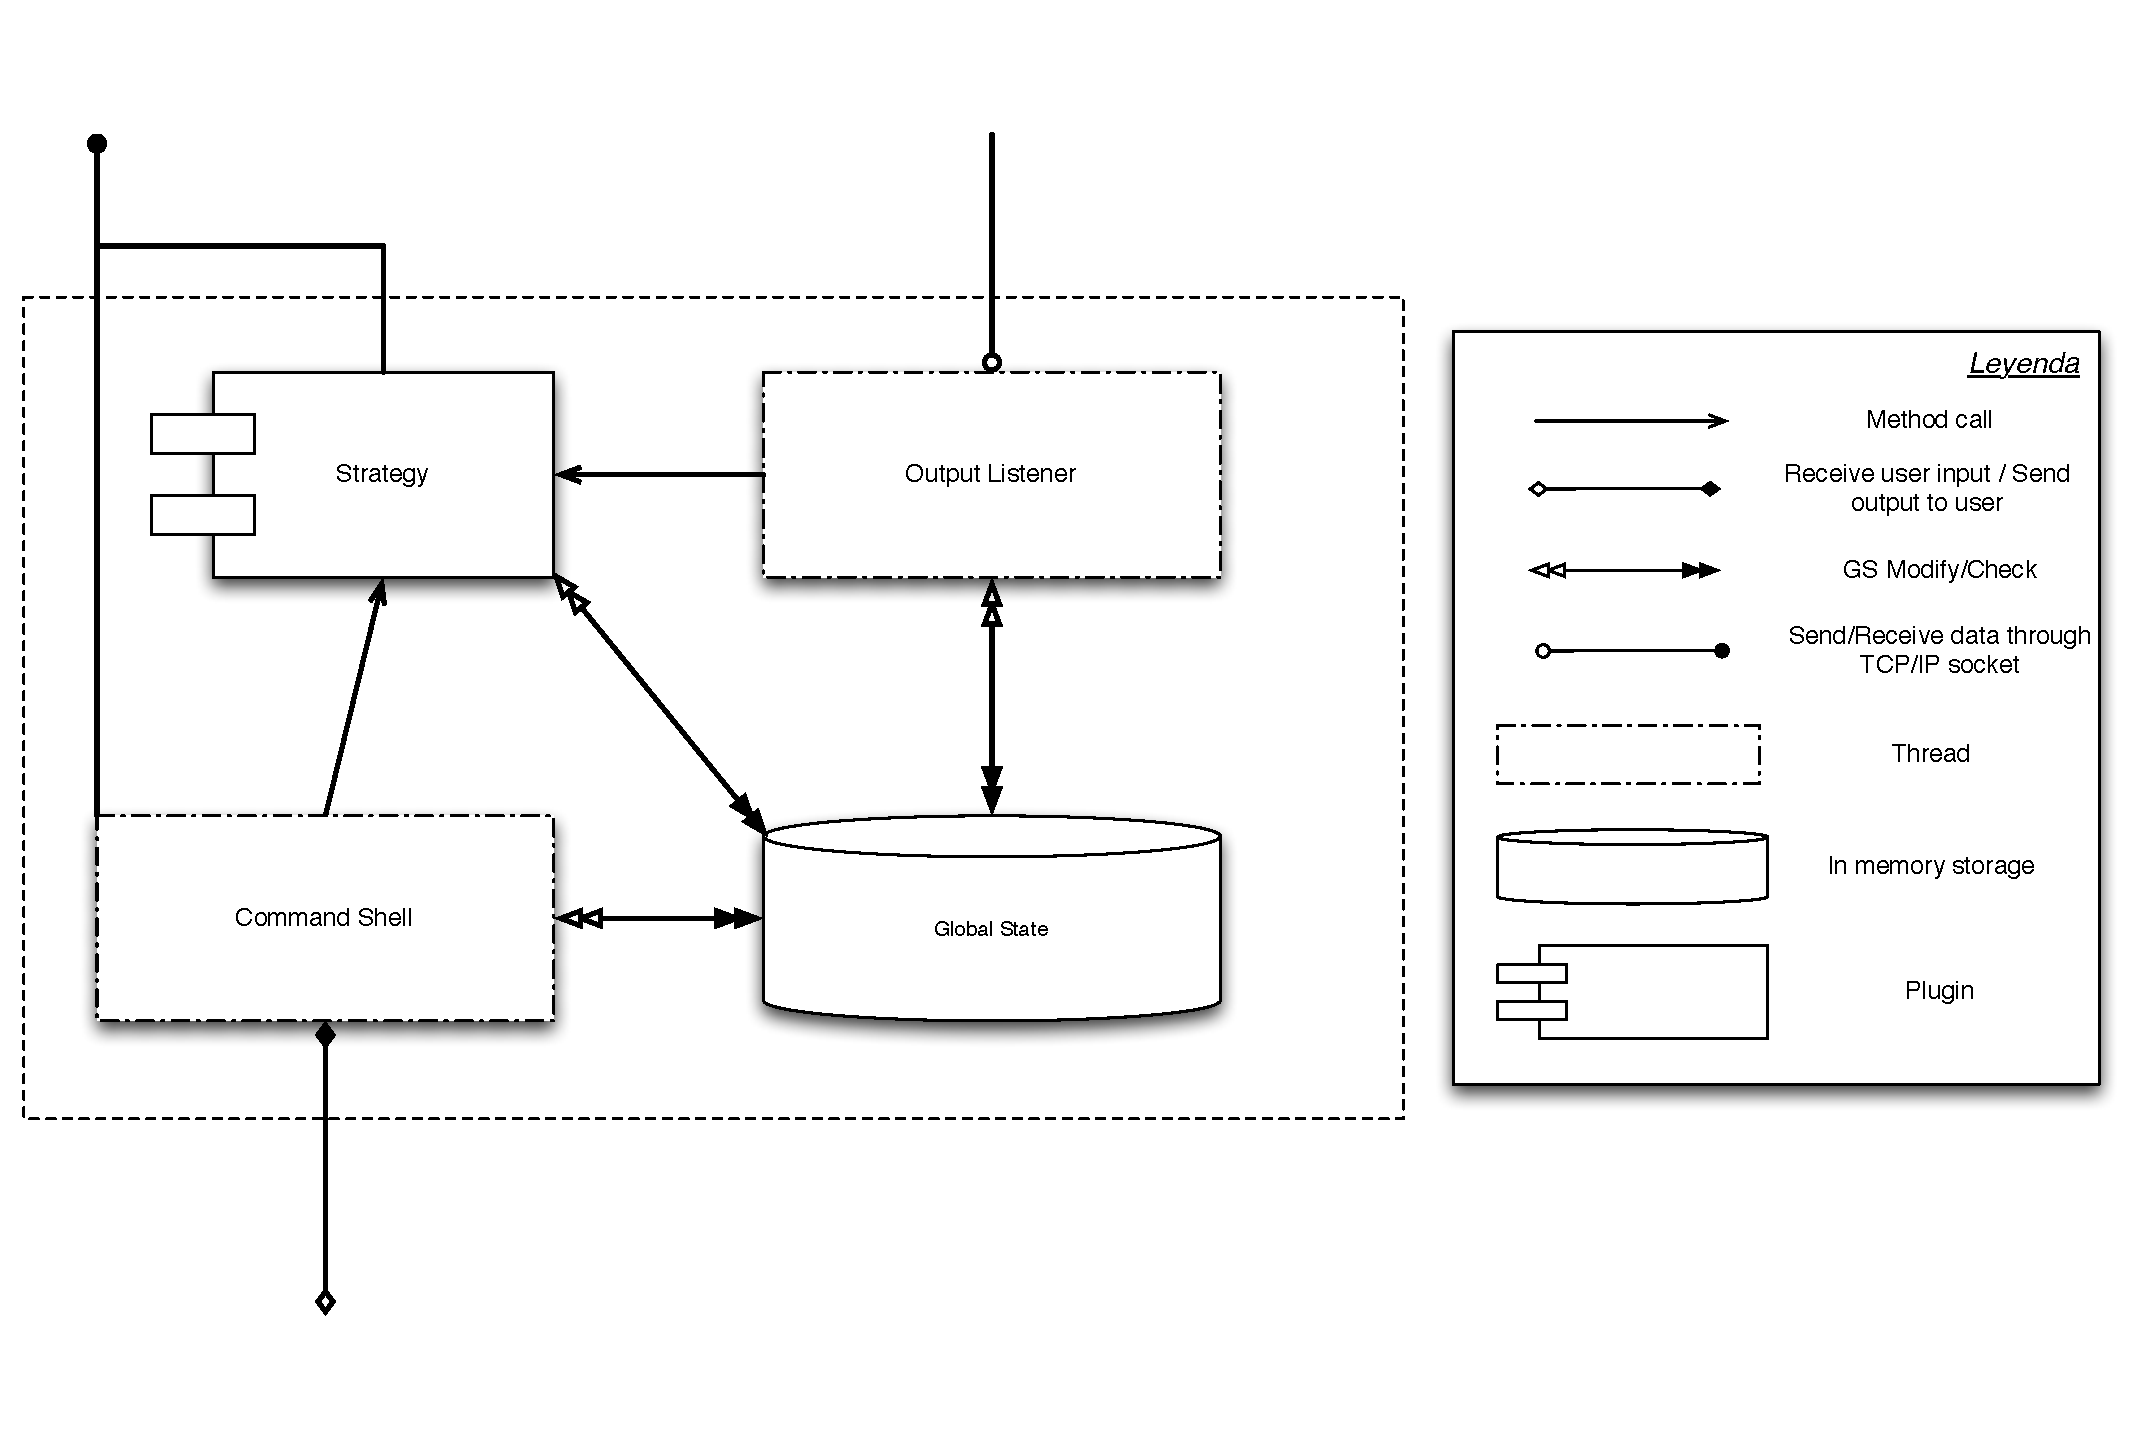
\includegraphics[scale=0.4]{graphs/frontend architecture}
\caption{Detalle de arquitectura del \fend}
\label{fig:frontend}
\end{figure}

\begin{wrapfigure}{r}{0.6\textwidth}
	\vspace{-3em}
	\begin{subfigure}{0.27\textwidth}
		\centering
		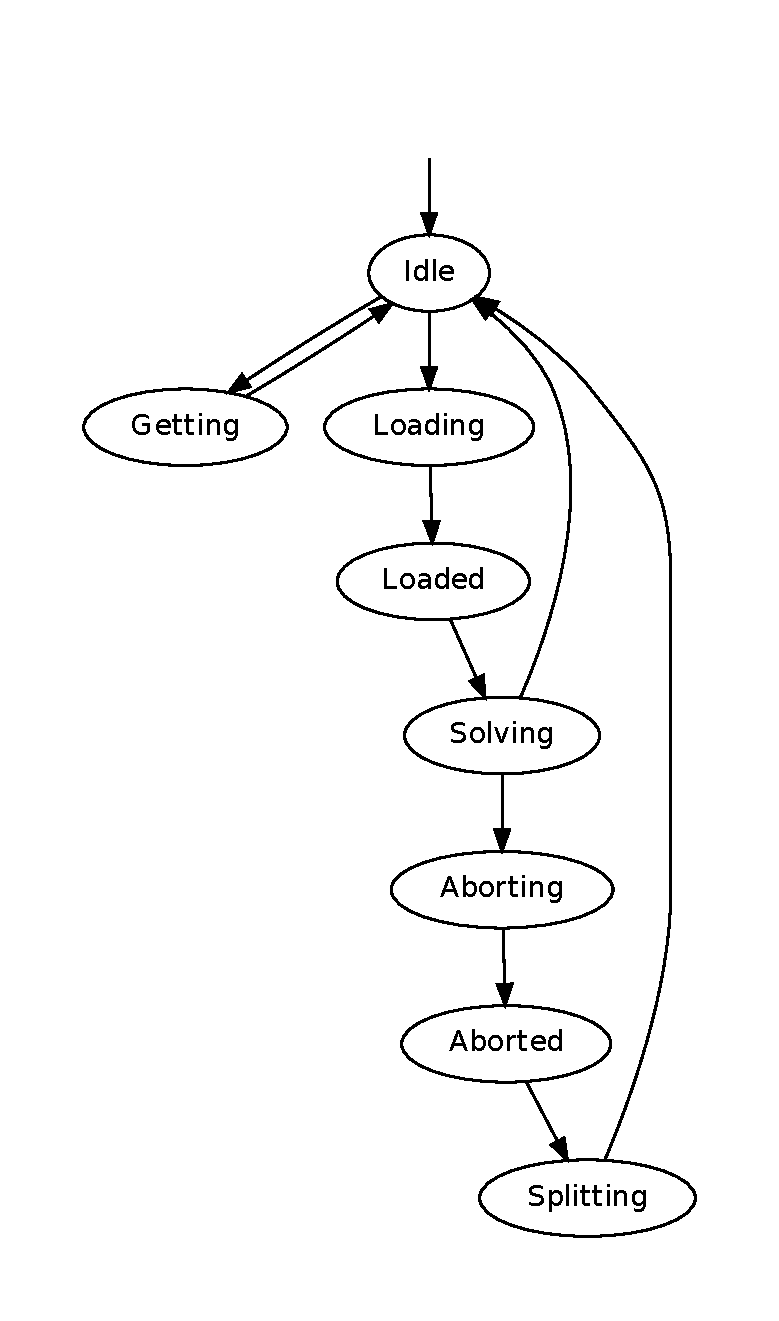
\includegraphics[scale=0.3]{graphs/workerstates}
		\caption{\emph{Workers}}
	\end{subfigure}
	\begin{subfigure}{0.27\textwidth}
		\centering
		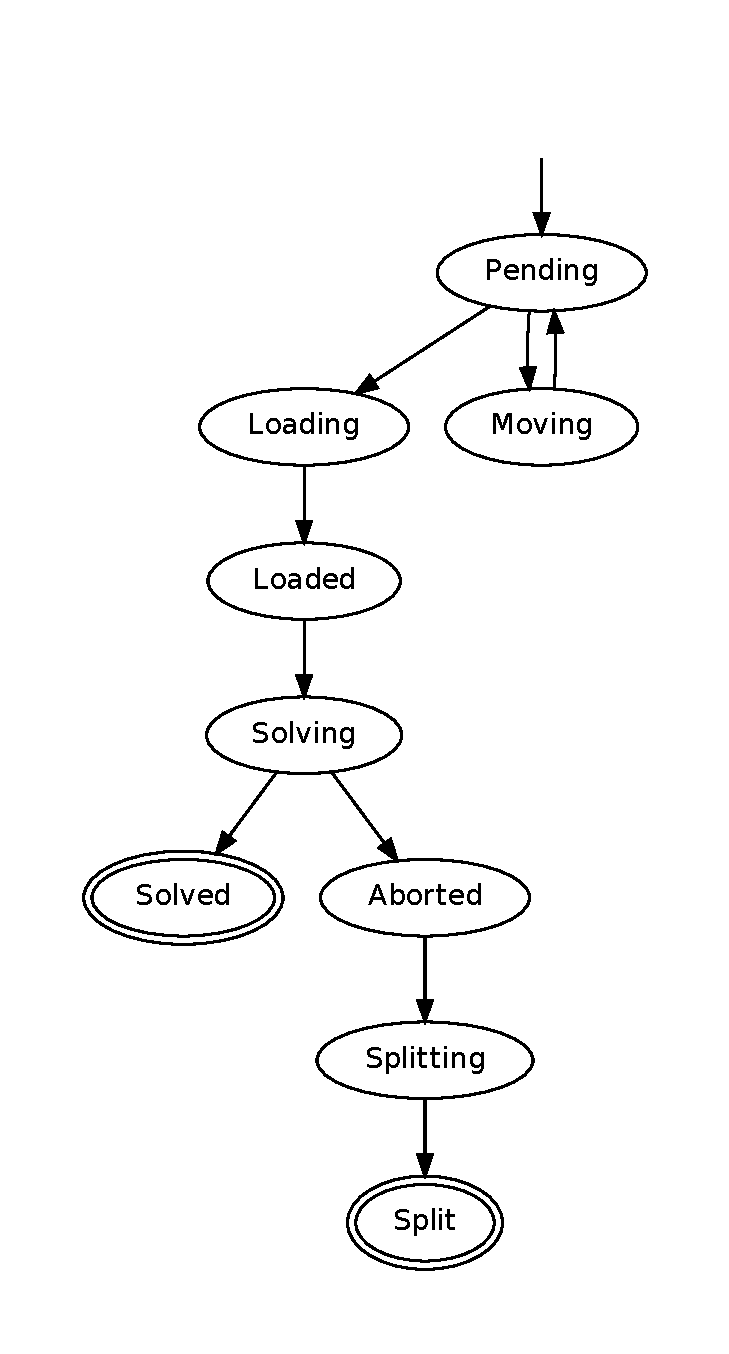
\includegraphics[scale=0.3]{graphs/taskstates}
		\caption{Tareas}
	\end{subfigure}
	\caption{Diagramas de estado en el tablero de control}
	\label{fig:states}
	\vspace{-1em}
\end{wrapfigure}

En la \fig\ref{fig:frontend} se esquematiza el diseño de componentes del
\fend. En esta figura se puede observar que el tablero de control proporciona
un modo doble de interacción con el \bend. Por un lado, el tablero de control
es capaz de recibir comandos del usuario en \rt a través de una interfaz de
tipo consola. Estos comandos representan acciones a ser llevadas a cabo en el
\bend como ser indicar a un \w ocioso que cargue una nueva tarea, indicar a un
\w que se encuentra trabajando en un problema que aborte dicha ejecución,
mover una tarea desde un \w a otro, etc. Por otro lado, el tablero de control
posee también una \emph{estrategia} (intercambiable) que permite llevar a cabo
acciones automáticamente frente a determinados eventos. El \fend posee también
un componente que procesa permanentemente la información que llega desde el
\bend. 

Es importante observar que todos los componentes mencionados comparten un
estado global. Esto se debe a que, tal como se explicó en la Sec.~\ref{sec:backend},
el \bend no tiene conocimiento del estado global del sistema. Por lo tanto, esta responsabilidad
recae en el \fend en la medida que este estado es necesario para poder tomar
decisiones ante los distintos eventos. El acceso concurrente a este estado
global nos obliga a introducir un mecanismo de sincronización entre los
distintos \threads de ejecución (\emph{locking}) que garantice la consistencia
del estado en todo momento. Hemos tenido el cuidado necesario para evitar que
el \emph{locking} atente contra la performance del componente en cuestión.

\begin{wrapfigure}{r}{.6\textwidth}
\vspace{-2em}
\begin{footnotesize}
\begin{lstlisting}[mathescape,language=Pascal,frame=single,label=lst:synchronouscmd,caption=Esquema de comando sincrónico]
DECIR_A $W$ que obtenga la tarea $T$
ESPERAR que tarea $T$ este en $W$
DECIR_A $W$ que cargue tarea $T$
ESPERAR que tarea $T$ este cargada
DECIR_A $W$ que comience a solvear $T$
\end{lstlisting}
\end{footnotesize}
\vspace{-3em}
\end{wrapfigure}

En la \fig\ref{fig:states} presentamos las máquinas de estado correspondientes
a los \ws y a las tareas. Estos diagramas esquematizan el estado que es
mantenido en el estado global del \fend. Una estrategia particular podría
requerir un estado más \emph{complejo} para tomar decisiones. Por ejemplo, se
podría requerir mantener cierta información histórica respecto de la
ejecución. En tal caso queda bajo exclusiva responsabilidad de la estrategia
la implementación de las estructuras de datos y algoritmos necesarios para
dicha tarea.


\begin{wrapfigure}{r}{.6\textwidth}
\begin{footnotesize}
\begin{lstlisting}[language=Python,caption=Interfaz Strategy,label=lst:strategy]
class Strategy(object):
	def register_globalstate(globalstate)
	def register_socket(commandsocket)
	def on_init(worker)
	def on_createroot(worker, task)
	def on_init_finished(nworkers)
	def on_getfile(worker, task)
	def on_file(worker, task)
	def on_load(worker, task)
	def on_unsat(worker, task)
	def on_sat(worker, task, modelstr)
	def on_abort(worker, task)
	def on_split_newtask(worker, newtask)
	def on_split_finished(worker, 
	                      parenttask, 
	                      nchildren)
	def on_shutdown()
\end{lstlisting}
\end{footnotesize}
\end{wrapfigure}

En cuanto a las estrategias, se siguió un modelo reactivo (\emph{eventos}).
Esto se debió en primera instancia a la dificultad de ejecutar secuencias de
comandos de forma sincrónica. Por ejemplo, si quisiéramos implementar la
obtención automática de una nueva tarea cuando un \w se queda sin tareas
pendientes y quisiéramos además que el \w comenzara a \solvear dicha tarea en
el momento en el que la misma esté disponible, deberíamos implementar un
algoritmo similar al expuesto en \lst\ref{lst:synchronouscmd}. El problema en
este algoritmo se encuentra en las líneas que comienzan con la palabra clave
\texttt{ESPERAR} ya que no es aceptable que la consola de comandos o la
estrategia se bloqueen a la espera de un evento que puede tardar una cantidad
arbitraria de tiempo en ocurrir. Esto se debe principalmente a que en el
transcurso de esa cantidad arbitraria de tiempo el \fend recibiría una
cantidad de información desde el \bend (por ejemplo, el hecho de que otro \w
terminó de \solvear el subproblema en el que estaba trabajando) que podría
requerir que se tomen acciones con el fin de mantener el sistema funcionando
eficientemente. Sin embargo, estas acciones no podrían ser tomadas porque el
\fend se encontraría bloqueado esperando a que un evento particular de un \w
particular ocurra. Ante este escenario optamos por un modelo de eventos que
presentamos en el \lst\ref{lst:strategy}. Esta interfaz modela el conjunto de
eventos que pueden ocurrir. Una estrategia particular debe implementar dicha
interfaz de modo de poder responder ante estos eventos.


%!TEX root = tesis.tex

\section{Sobre la automatización}

En la presente sección nos proponemos señalar los aspectos importantes a tener
en cuenta relacionados con la automatización del funcionamiento de nuestra
herramienta. Además señalaremos las decisiones adoptadas por nosotros en cada
uno de los puntos relevantes.

\subsection{Consideraciones sobre la estrategia}

Comenzaremos esta sección desglosando las principales cuestiones a
resolver por una estrategia completamente automática para nuestra herramienta.
Surge así la primer pregunta relevante que cualquier estrategia debe
responder: ¿Cuándo declarar que un (sub)problema es demasiado difícil para
atacarlo como tal? Es decir: ¿Cuándo se toma la decisión de partir un problema
en nuevos subproblemas?

\subsubsection{Dificultad de un problema}

En este punto es importante destacar el hecho de que la partición de un
problema en nuevos subproblemas se lleva a cabo con el objetivo de distribuir
las distintas porciones del espacio de búsqueda entre distintas unidades de
cómputo. Así, invertir demasiado tiempo en intentar obtener un resultado
secuencialmente para un problema difícil atenta prohibitivamente contra el
paralelismo. Por lo tanto la decisión de cuándo abortar un \solving en curso
se vuelve crucial.

Si un problema va a tomar demasiado tiempo no tiene sentido invertir tiempo de
\solving secuencial en intentar resolverlo y es conveniente partirlo
\emph{cuanto antes}. Por otra parte, partir un problema en un momento tal que
si hubiéramos esperado una fracción  pequeña de tiempo más el \w habría
arribado a un resultado para el problema implica que \emph{todo} el tiempo de
cómputo previamente invertido es desperdiciado. Estos dos errores se vuelven
catastróficos cuando se repiten en forma sistemática sobre los subproblemas a los que un problema da origen.

Subyace a toda esta cuestión la pregunta fundamental de cómo determinar que un
problema dado es fácil o difícil. Si tuviéramos algún criterio que nos
permitiese siquiera aproximar la dificultad de un problema dado, o el
porcentaje de avance durante una corrida secuencial de un \ssolver, podríamos
elaborar una estrategia que atienda razonablemente a las inquietudes
planteadas arriba. Lamentablemente no se conoce ninguna métrica que permita
establecer \apriori la dificultad de un problema. Si bien la complejidad de
los algoritmos de \ssolving se expresa en función de la cantidad de variables
de un problema (y es exponencial), la experiencia indica que existen problemas
con pocas variables sumamente difíciles y problemas con muchas variables
razonablemente sencillos.

\subsubsection{Cuándo partir: criterios estáticos vs. dinámicos}

Resulta claro entonces que una primera aproximación \emph{naive} a este
problema, como por ejemplo la elección de un \tout fijo a modo de criterio para
determinar cuándo un problema debe ser partido, resulta una mala alternativa.
La disparidad en la dificultad de los distintos problemas hace imposible
dar con un único valor prefijado de \tout que resulte adecuado para el
caso general. Otra posibilidad sería entonces que el usuario seleccionara
el \tout deseado para cada problema. Sin embargo, esto atenta sustancialmente
contra la usabilidad de la herramienta, ya que requiere asumir un \emph{expertise} por
parte del usuario y un conocimiento previo del problema a resolver que no son
razonables.

Además, a medida que partimos recursivamente un problema, los subproblemas
generados --si la elección de variables a levantar fue apropiada-- son
\emph{cada vez} más fáciles. Por lo tanto un valor de \tout que resulte
adecuado en cierto momento ya no lo será más adelante. Esto podría llevarnos a
elaborar un criterio un tanto más refinado que lo anterior. Por ejemplo,
podríamos optar por tener un valor de \tout para cada \emph{nivel} del
problema. Sin embargo, surge nuevamente el mismo inconveniente: cada vez
que un problema es partido, los subproblemas generados difieren notablemente
en su nivel de dificultad. Más aún, las distribuciones de dificultad entre
los hijos de dos subproblemas distintos de un mismo problema (a misma cantidad
de variables levantadas) pueden ser muy distintas. En consecuencia, este
refinamiento tampoco resulta adecuado.

En general, la ausencia de un criterio estático para determinar la dificultad
de un problema dado hace imposible la elección de un criterio de corte que
sea también estático. Por lo tanto se vuelve necesario que el criterio para
determinar que un problema debe ser partido sea dinámico. Es decir, que el
mismo se vaya adaptando durante la ejecución. Un criterio de estas
características tiene dos fuentes de información fundamentales. Por un lado el
estado general del sistema y su evolución (su historia). Esto puede incluir
métricas sobra la carga del sistema, cantidad de problemas pendientes, espacio
de almacenamiento disponible, etc. La segunda fuente de información surge de
las características del problema que sean observables a lo largo de la
ejecución. Ejemplos de esto son la cantidad de subproblemas producidos cada
vez que se partió un problema, estadísticas sobre los tiempos que demoraron
los subproblemas ya resueltos, etc. 

Cualquier estrategia automática razonable deberá entoces dar respuesta a la
problemática de decidir cuándo partir un problema teniendo en cuenta las
observaciones mencionadas. Una vez resuelto este dilema surge la segunda
pregunta fundamental a responder que es: ¿Cómo partir un problema? Que
esencialmente se traduce en: ¿Cuántas y qué variables levantar en cada ocasión?

\subsubsection{Cómo partir: criterios de selección de variables}

\newcommand{\vsids}{VSIDS\xspace}

La determinación de qué variables levantar en el momento en que se decide
partir un problema es uno de los grandes temas en el mundo del \ssolving. En
un sentido, este problema es equivalente al problema que enfrentan los
\ssolver secuenciales cuando deben tomar una decisión. Cuando un \ssolver
secuencial agotó las propagaciones de la última decisión tomada, debe tomar
una nueva decisión. Tomar una decisión implica en primera instancia
seleccionar una variable y luego seleccionar cuál de los dos posibles valores
de verdad asignar a esa variable. En nuestro caso, dado que al levantar una
variable los dos valores de verdad son considerados \emph{simultáneamente}, el
problema se reduce a elegir cuidadosamente la variable a levantar. Uno de los
métodos más difundidos para elegir la próxima variable en los \ssolvers
secuenciales, se basa en un criterio de actividad conocido como \vsids. Del
mismo modo que para las cláusulas --ver Sec.~\ref{sec:longactlbd}-- cada vez que
una variable \emph{participa} de un conflicto su actividad es incrementada.
Luego, cuando el \ssolver se encuentra en la situación de tener que elegir una
variable para continuar la búsqueda, elige aquella con mayor actividad.

La elección de las variables a ser levantadas es crucial. Como se ve en
la Tabla~\ref{distrospamela8}, una buena elección de variables puede generar una
descendencia muy fácil o muy difícil. En general, no es posible predecir cuál es
la mejor elección de variables a ser levantadas. Sin embargo la heurística
\vsids ha reportado muy buenos resultados en el mundo del \ssolving secuencial.


\begin{table}
\begin{footnotesize}
\begin{tabular}{ccrrrrr}
\toprule
Subconjunto & Cant. hijos & & & & & \\
de variables & no triviales & M\'aximo & Media & Suma total & Desv.
est. & Mediana \\
\cmidrule(r){1-7}
A 	& 136 	& 8.09 		& 1.13 		& 154.17	 	& 1.37 		& 0.51 \\
B 	& 136 	& 18.06 		& 1.28 		& 173.48	 	& 1.95 		& 0.72 \\
C 	& 192 	& 36.25 		& 8.74 		& 1678.88 	& 7.45 		& 5.78 \\
D	& 174 	& 63.62 		& 1.25 		& 218.29	 	& 6.27 		& 0.05 \\
E	& 192 	& 89.41 		& 2.18 		& 418.04	 	& 7.66 		& 0.39 \\
F 	& 192 	& 288.79	 	& 10.18 		& 1954.07 	& 22.36 		& 2.46 \\
G 	& 256 	& 376.70	 	& 86.03 		& 22024.53 	& 81.98 		& 56.98 \\
\bottomrule
\end{tabular}
\end{footnotesize}
\caption{Ejemplo: siete elecciones de variables distintas para partir un mismo problema. Tiempos secuenciales, en segundos, para los subproblemas resultantes de cada partición.}\label{distrospamela8}
\end{table}


Además de la determinación de qué variables levantar, es importante también
tener en cuenta cuántas levantar en cada momento. En primer lugar, es
importante tener en cuenta que la cantidad potencial de subproblemas generados
es exponencial con respecto a las variables levantadas. Esto afecta en un
doble sentido. En primera instancia es necesario observar que, dado que el
proceso de particionado se repite recursivamente, la generación de una
excesiva cantidad de subproblemas ante cada particionado genera una explosión
exponencial de problemas. Si este factor no es tenido en cuenta es altamente
probable que el sistema diverja y no sea capaz de arribar a una solución.
Sumado a esto, el tiempo insumido en generar los subproblemas producto de un
problema puede volverse excesivamente grande atentando una vez más contra el
paralelismo y la eficiencia de la herramienta.

Una vez más debemos recordar que la idea de levantar variables se basa en que,
ante una elección razonable de cuáles variables levantar, a mayor cantidad de
variables levantadas, más fáciles serán los subproblemas generados. Es por
esto que si la cantidad de variables a levantar es demasiado pequeña, es
probable que los subproblemas que sean generados no sean suficientemente 
fáciles como para ser resueltos y que, por lo tanto, sea necesario partirlos también en el
futuro haciendo que el tiempo invertido en intentar resolverlo se convierta en
tiempo desperdiciado. Además, si la cantidad de variables levantadas es muy
baja, existe la posibilidad de que la cantidad de subproblemas generados no
sea suficiente para aprovechar al máximo el \hard disponible.

La última observación referida al criterio de particionado tiene que ver con
qué problemas son dignos de ser distribuidos realmente. Hemos mencionado
muchas veces que al levantar $n$ variables, la cantidad \textbf{potencial} de
subproblemas generados es $2^n$. El uso de la palabra potencial tiene que ver
con el hecho de que varios de los subproblemas generados al levantar $n$
variables podrían ser resueltos trivialmente ¿A qué nos referimos con
trivialmente? En primer lugar a aquellos subproblemas en los que alcanza con
propagar\footnote{El uso del término propagación en este contexto es estricto.
Es decir que nos referimos exclusivamente a la realización de la clausura de
\bcp sobre el subproblema. Esta propagación no incluye la toma de nuevas
decisiones.} las implicaciones de las decisiones tomadas para obtener un
resultado --\sat o \unsat--. Pero más en general, nos referimos a todos
aquellos subproblemas en los que el \emph{overhead} de generar la tarea,
trasladarla a otro \w, cargar la tarea en el nuevo \w, y \solvear dicho
problema hasta arribar a un resultado sea suficientemente grande como para que
sea conveniente resolverlo directamente sin generar
una nueva tarea.

Se introduce entonces una nueva variable en el criterio de particionado que es
cuáles de los potenciales $2^n$ subproblemas generar como tareas a ser
resueltas por otros \ws y cuáles resolver directamente sin generarlos como nuevas
tareas. Se debe observar que \emph{no generar} un subproblema requiere invertir
un tiempo de cómputo suficiente para determinar el resultado de ese
subproblema. Una estrategia automática debe entonces decidir qué hacer con
esta variable teniendo en cuenta que invertir poco o nada de tiempo de cómputo
en filtrar los subproblemas puede degradar significativamente la eficiencia
del sistema debido a que una cantidad de subproblemas
demasiado fáciles serán generados como nuevas tareas. Pero también debe tener en cuenta que invertir demasiado
tiempo de cómputo en el filtrado de los subproblemas tiende a degradar
significativamente el paralelismo.

\subsubsection{Otros aspectos de interés}

Otro aspecto que influye en la \emph{performance} de la herramienta es la
forma en que se recorre el espacio de búsqueda. Cuando un \w queda ocioso debe
tomar una nueva tarea (si hubiera tareas pendientes). Surge entonces el
problema de determinar cuál de todas las tareas pendientes debe ser resuelta.
Como en los casos anteriores existen dos factores que deben ser balanceados.
Por un lado, si la estrategia (i.e. toma automática de decisiones) es adaptable según ciertas métricas sensadas dinámicamente, el
orden en el que se recorren las tareas a resolver alterará el resultado. Luego, nos gustaría poder
forzar a la herramienta a seguir el orden \emph{más adecuado} en relación a dichas métricas. En este contexto, la tarea \emph{ideal} puede encontrarse
almacenada en otro \w. Surge así el segundo factor a tener en cuenta. En aras
de la escalabilidad, el criterio para elegir la próxima tarea a ser resuelta no
debe generar una sobreutilización de la red de comunicaciones.

Un último factor a tener en cuenta es la necesidad de maximizar la utilización
del \hard disponible. Es decir que, idealmente, si hay \hard ocioso no debería
haber tareas pendientes, aún cuando estas se encuentren almacenadas en otros \w.

\subsection{La estrategia implementada}
\label{estrategia:implementada}

Teniendo en cuenta los factores mencionados anteriormente nos volcamos al
desarrollo de una estrategia automática. Nuestro objetivo no estuvo puesto en
el desarrollo de una estrategia óptima ya que cada uno de los factores
mencionados con anterioridad podría ser objeto de un extenso y minucioso estudio. 
Más aún, no existen garantías de que tal estrategia óptima exista. Por lo tanto nuestro esfuerzo estuvo dedicado a no
incurrir en los errores más flagrantes, de modo que la herramienta funcionase
razonablemente bien con una serie de problemas y poder empezar a obtener
resultados que nos permitan resaltar los aspectos fuertes y los aspectos que
aún necesitan un esfuerzo importante.

En cuanto al criterio de particionado las decisiones tomadas fueron:

\begin{itemize}
	\item La cantidad de variables a levantar se fijó en 10. Aunque este valor puede ser alterado por el usuario.
	\item Las variables a levantar se seleccionan utilizando la heurística \vsids. Es decir que cuando un problema va a ser partido, se consulta la actividad de cada variable y se seleccionan --de acuerdo con el punto anterior-- las diez más activas.
	\item Cada potencial subproblema es \solveado por 50ms. Si en ese tiempo no se arriba a un resultado, se genera una nueva tarea pendiente.
\end{itemize}

Respecto al orden en el cual se recorre el espacio de búsqueda:

\begin{itemize}
	\item Si un \w queda ocioso y no tiene tareas pendientes en su espacio de almacenamiento, obtiene la tarea que corresponda de acuerdo al recorrido BFS --\emph{breadth-first search}-- del árbol de que representa el espacio de valuaciones aún no explorado.
	\item Si al quedar ocioso el \w cuenta con tareas pendientes en su espacio de almacenamiento, se selecciona la que corresponda por BFS de las tareas locales.
\end{itemize}

Sobre cuándo declarar que un problema es demasiado difícil, adoptamos una
estrategia basada en el estado del sistema. En concreto nos enfocamos en que
el sistema mantenga una cierta tasa de progreso. Para ello medimos la cantidad
de subproblemas resueltos por unidad de tiempo y luego establecimos un umbral
objetivo. De esta forma, si la frecuencia actual se encuentra por debajo del umbral
objetivo, entonces debemos escojer uno de los problemas que actualmente están
siendo resueltos y partirlo.

Llamaremos \textbf{frecuencia objetivo} al umbral, entendido como 
cantidad de problemas resueltos por \w, por segundo por debajo del cual se decide que algún
problema debe ser partido. Llamaremos \textbf{frecuencia actual} a un valor
que estima la cantidad de problemas terminados por \w, por segundo a partir de
promediar los problemas que han terminado durante los últimos $t$ segundos.
Llamaremos \textbf{tamaño de la ventana de muestreo} al mencionado valor $t$.
Llamaremos \textbf{frecuencia de observación} a la frecuencia con la que se revisa
si la frecuencia actual se encuentra por encima de la frecuencia objetivo.

En concreto los parámetros utilizados fueron:

\begin{itemize}
	\item Frecuencia objetivo: $0.15$ p/\w p/seg.
	\item Tamaño de la ventana de muestreo: $20s$
	\item Frecuencia de observación: cada $5s$
\end{itemize}

Que la frecuencia objetivo dependa de la cantidad de \ws permite ajustar la
cantidad de problemas generados de acuerdo a la capacidad de consumirlos que
tiene el sistema. Es importante notar que el tamaño de la ventana influye en
cuánto peso se le da a la historia. Tomar una ventana de mayor tamaño exhibirá un comportamiento más estable en el tiempo,
mientras que una ventana más pequeña se adapta más rápidamente y consecuentemente mostrará mayor variabilidad. La frecuencia de observación administra cuánto tiempo de
tolerancia se tiene ante una frecuencia actual menor a una frecuencia
objetivo. Si la frecuencia de observación es alta --menor valor-- entonces la
tolerancia será baja y ante cualquier caída de la frecuencia actual por debajo
del objetivo el sistema reaccionará. Por otro lado, una frecuencia baja --mayor
valor-- representará una tolerancia mayor, dando oportunidad al sistema de
tener períodos en los que la frecuencia actual no alcance la frecuencia
objetivo. La combinación de estos tres parámetros configura la agresividad
del sistema a la hora de determinar que un problema es demasiado difícil.

Además del criterio por frecuencia decidimos que, ante la situación en la que hay
\ws sin tareas para realizar y en el sistema no hay más tareas pendientes, se
debe partir un problema en curso. De este modo evitamos que haya recursos
ociosos. En particular esta decisión es útil al comienzo de la ejecución de un
problema para distribuir rápidamente el trabajo entre las distintas unidades
de cómputo.

Falta determinar entonces cuál de los problemas en curso será el seleccionado
para ser partido. En este punto optamos por aquel en el que se ha
invertido más tiempo de cómputo. De este modo evitamos que un \w quede atorado
intentando resolver un problema que podría ser extremadamente difícil, a la vez
que procuramos evitar que un problema sea partido demasiado pronto.

Con respecto al balanceo del almacenamiento se tomó la decisión de que cada
vez que un \w queda ocioso y sin tareas locales pendientes, además de obtener la
tarea que corresponde por BFS, el \w obtendrá una conjunto de tareas pendientes
de aquel \w que posea mayor cantidad. Llamemos $w_{idle}$ al \w que quedó sin
tareas y $w_{overwhelmed}$ al que más tareas pendientes posee, entonces la
cantidad de tareas transferidas en esta ocasión será:

\begin{equation}
\frac{\#tareas\_pendientes(w_{overwhelmed})}{\# workers}
\label{eq:share}
\end{equation} 

La idea detrás de esto es que $w_{idle}$
obtiene \emph{la porción que le corresponde} de las tareas de
$w_{overwhelmed}$. Para evitar transferencias extremadamente largas, la
cantidad expresada en Eq.~\ref{eq:share} satura en $10$ tareas. Para evitar
una mala distribución, las tareas que conforman una porción a ser transferida
son seleccionadas al azar del conjunto de tareas pendientes de
$w_{overwhelmed}$. Vale la pena notar que si un \w solicitara las $n$ tareas que mejor califican según el criterio de elección, éste concentraría un conjunto de tareas de alta prioridad, generando un potencial problema de contención.

\section{Resultados experimentales}

En esta sección presentamos los experimentos realizados con el fin de evaluar
el desempeño de nuestra herramienta.  Los experimentos se ejecutaron en el
\cluster CeCAR\footnote{Centro de C\'omputos de Alto Rendimiento de la FCEyN. \url{http://cecar.fcen.uba.ar/}}.
Se utilizaron 17 equipos,
cada uno de los cuales cuenta con dos procesadores \texttt{Intel Dual Core Xeon
5030 2.67 Ghz}, \texttt{2 GB} de memoria RAM y un disco rígido \texttt{Western
Digital WD800JD 80Gb SATA 7200RPM}. Uno de los equipos fue utilizado para
ejecutar el tablero de control y el \master, mientras que se ejecutaron 4 \ws
en cada uno de los restantes 16 equipos totalizando 64 \ws.


\subsection{Casos de estudio}

Debido a la orientación del grupo de investigación, nos interesa evaluar la herramienta principalmente en lo que respecta a su uso para la verificación formal de software. En la práctica, nos interesa hacerlo sobre todo para problemas resultantes de la traducción de especificaciones de sistemas y propiedades en el lenguaje Alloy; esto es, de modo de evaluar la viabilidad de usar la herramienta para capitalizar la disponibilidad de \emph{hardware} ocioso y reemplazar el uso de la herramienta secuencial Alloy Analyzer en aquellos casos en que esta última demora demasiado en demostrar una propiedad (o en que sus capacidades directamente se ven excedidas, de modo que el problema no resulta tratable en secuencial).

Otro aspecto de los problemas difíciles provenientes de especificaciones Alloy que resulta interesante para conformar un \emph{benchmark} es que pueden ser generados en distintos grados de dificultad a medida que se elevan las cotas para los dominios de datos atómicos sobre los que predican. Como se mencionó en el Cap.~\ref{intro}, para que el análisis resulte decidible se procede a acotar dichos dominios (así, las propiedades se demuestran automáticamente pero, por ejemplo, ``\ldots para hasta 12 trenes, 8 semáforos y 8 pasos a nivel''). En el caso de Alloy, estas cotas suelen denominarse \emph{scopes}. En otras palabras, el problema de verificar cierta propiedad sobre cierto modelo da origen a una sucesión o familia de problemas (para \emph{scopes} cada vez mayores) que son estructuralmente similares pero ostentan cantidades de variables, cláusulas y tiempos de \emph{solving} secuencial estrictamente crecientes.

Otra potencial fuente de problemas que resulta natural considerar son los \emph{benchmarks} de las competencias anuales de \ssolving. Sin embargo, la forma en que tradicionalmente se evalúan las herramientas en dichos eventos consiste en medir, para cada \ssolver $S$ y para cada cantidad de tiempo $t$, la \emph{cantidad} de problemas que $S$ logra resolver en $t$ segundos. (Esto se debe a que algunos problemas fáciles para un \emph{solver} son difíciles para otros y viceversa.) En consecuencia, los \emph{benchmarks} de las competencias suelen incluir gran cantidad de problemas muy pequeños, pequeños y medianos cuyo tratamiento optimizado escapa al alcance de nuestra herramienta.


\subsubsection{\emph{Garbage collection} usando Mark \& Sweep}

Entre los casos de estudio provistos con el programa Alloy Analyzer se incluye un modelo formal de una implementación de \emph{garbage collection} basada en el algoritmo conocido como ``mark and sweep''. El modelo incluye una representación del \emph{heap} del sistema, dominios de datos \texttt{HeapState} y \texttt{Node}, una especificación del algoritmo y propiedades \texttt{Soundness} y \texttt{Completeness}.

La propiedad de \texttt{Soundness} afirma que, tras haber ejecutado el algoritmo de \emph{garbage collection}, no hay intersección entre el conjunto de nodos alcanzables en el \emph{heap} y la lista de nodos libres. La propiedad de \texttt{Completeness} afirma que, tras haber ejecutado el algoritmo, todo nodo inalcanzable en el \emph{heap} efectivamente aparece en la lista de nodos libres.

Hemos incluido ambos problemas en el \emph{benchmark} para la evaluación de la herramienta. Ambos son problemas difíciles que requieren exponencialmente más tiempo de análisis conforme crece la cantidad de \texttt{Node}s en el \emph{scope}. Sin embargo, el segundo problema (el de demostrar \texttt{Completeness}) exhibe una curva de dificultad aún más pronunciada que el primero.


\subsubsection{Ruteo en redes heterogéneas}

Este caso proviene de un modelo formal de ruteo en redes heterogéneas, desarrollado en AT\&T, que involucra agentes móviles, identificadores, rutas y múltiples dominios de red. El modelo en cuestión incluye diversas propiedades, de las cuales la última, \texttt{StructureSufficientForPairReturnability}, resulta particularmente costosa de demostrar. Para más detalles referimos al lector al artículo ``Compositional Binding in Network Domains'' \cite{zave:fm06}.


\subsubsection{Clausura relacional reflexo-transitiva}

Se trata de un modelo sencillo que involucra un dominio de datos $A$ y una relación $R \subseteq A \times A$, a la que (sólo) se le exige que sea reflexiva y transitiva. La propiedad a verificar afirma que $R^{*} = R$, esto es, que la clausura reflexo-transitiva de una relación reflexiva y transitiva es exactamente esa relación. Esta es una propiedad válida, cosa que podría probarse matemáticamente, por fuera del modelo. El interés radica en que se trata de un modelo breve y sencillo cuya traducción engendra problemas con cantidades muy pequeñas de variables proposicionales, pero que a pesar de ello resultan de considerable dificultad para los \ssolvers y exhiben una curva exponencial (tiempo de \solving para $|A|$ creciente) relativamente pronunciada.


\subsection{Resultados obtenidos}


La Tab.~\ref{tab:resultados} muestra la comparación entre el tiempo de
ejecución requerido por el \ssolver secuencial (columna ``seq.~walltime~(s)'')
y el tiempo percibido requerido por nuestra herramienta (columna
``avg.~par.~walltime~(s)''). Los tiempos reportados para el caso distribuido
se calcularon tomando el promedio de varias corridas. La columna ``reps''
indica la cantidad de repeticiones realizadas para cada problema. La columna
``speedup'' es el resultado de la siguiente división:
$$\frac{\text{seq.~walltime~(s)}}{\text{avg.~par.~walltime~(s)}}$$ Este valor
denota la mejora relativa obtenida mediante la utilización de nuestra
herramienta. La columna ``efficiency'' es el resultado de la siguiente división:
$$\frac{\text{speedup}}{\text{\#\ws}}$$
Esta medida indica la ganancia neta de \emph{speedup} por \w utilizado.

\begin{table}
	\footnotesize
	\begin{tabular}{lrrrrrr}
		\toprule
		problem	&	scope	&	seq. walltime (s)	&	reps. & avg. par.	&	speedup	&	efficiency \\
			&		&	&	 & walltime (s)	&		&	 \\
		\cmidrule(r){1-7}
		Routing	&	8	&	308.26	&		7 & 60.46	& 5.10x	&	0.08 \\
		Routing	&	9	&	76168.16	&	6& 407.34	& 	186.99x	&	2.92 \\
		Routing	&	$^*$10	&	$>$1209600.00	&	5 & 5046.84	&	$>$239.67x	&	$>$3.74 \\
		\cmidrule(r){1-7}
		Closure	&	11	&	749.65	&	14 & 291.28	&	2.57x	&	0.04 \\
		Closure	&	12	&	3983.36	&	5 & 1914.45	&	2.08x	&	0.03 \\
		Closure	&	13	&	16261.35	& 5 &	4362.61	&	3.73x	&	0.06 \\
		\cmidrule(r){1-7}
		GC Soundness2	&	9	&	217.31	&	10 & 200.85	&	1.08x	&	0.02 \\
		GC Soundness2	&	10	&	 2855.30	&	7 &1376.89	&	2.07x	&	0.03 \\
		\cmidrule(r){1-7}
		GC Completeness	&	8	&	180.25	&	7 & 61.50	&	2.93x	&	0.05 \\
		GC Completeness	&	9	&	18643.06	&	5 & 1825.60	&	10.21x	&	0.16 \\
		\bottomrule
		\\
		\multicolumn{7}{l}{\begin{tiny}$^*$: Se ejecutó por 14 días sin que el \ssolver secuencial consiga un resultado\end{tiny}}
	\end{tabular}
	\caption{Tiempo de ejecución (en segundos) distribuido vs. secuencial}
	\label{tab:resultados}
\end{table}

En primera instancia corresponde aclarar por qué la cantidad de repeticiones
realizadas para cada problema son diferentes. Esto se debe a que procuramos
realizar la mayor cantidad de repeticiones posibles para cada problema. Por lo
tanto, la cantidad de repeticiones para los problemas más grandes fue menor
que la de los problemas más pequeños.

Una de las hipótesis de trabajo es la disponibilidad de \hard y, en
particular, la de \emph{clusters} de cómputo intensivo que pueden ser usados
para validar y/o verificar software.

Respecto a los resultados obtenidos, el \emph{speedup} que se exhibe en la
tabla, tal como lo evidencian los datos consignados en la columna
\emph{efficiency}, a menudo dista considerablemente del ideal si se considera
que es resultante de utilizar 17 unidades de cómputo. Sin embargo debe
destacarse que:

\begin{itemize}
\item en general el \emph{speedup} es creciente respecto del tamaño de los problemas que conforman el \emph{benchmark}, indicando esto que el enfoque resulta apropiado para resolver problemas de gran tamaño que no son tratables en el contexto de \ssolving secuencial,
\item si exceptuamos los casos extremadamente positivos --Routing--, y el caso GC Soundness2 para scope 9 en el que la mejoría percibida es muy baja, el rendimiento del enfoque reporta una ganancia mínima de $2.07x$, promedio de $4.35x$ y una ganancia máxima de $10,21x$.
\end{itemize}

\subsubsection{Uso de recursos en componentes centralizadas}

En la Sec.~\ref{sec:arquitectura} presentamos la arquitectura de la
herramienta. En ella puede observarse que existen dos puntos centralizados de
carga: el \master y el Tablero de control. Cabe entonces preguntarse si
estos puntos centralizados no representan una amenaza a la capacidad del
sistema de incorporar más unidades de cómputo en el futuro.

La Tabla~\ref{tab:incremental} muestra el impacto que tiene el agregado de
nuevas unidades de cómputo sobre el desempeño del nodo en el que fueron
ejecutados tanto el \master como el Tablero de control. En los datos consignados se
puede observar que el impacto de estas componentes en la carga y en el uso de
memoria del sistema son (y se mantienen) extremadamente bajos. Si bien lamentablemente
no pudimos contar con grandes cantidades de nodos adicionales para garantizar
que estos resultados se mantengan a gran escala, la tendencia parece confirmar
que es posible incrementar considerablemente la cantidad de unidades de cómputo
utilizadas sin que las componentes en cuestión se conviertan en un factor limitante.

%Cabe mencionar que este nodo, y las tareas que realiza, son los únicos potenciales cuellos de botella
%que presenta la herramienta. De los datos consignados se puede observar no
%sólo una utilización objetivamente muy baja de los recursos disponibles en
%dicho nodo, sino que el agregado de nuevos \w de cómputo no exhibe un
%crecimiento que ponga en riesgo la escalabilidad de la herramienta.

\begin{table}
	\centering
	\begin{tabular}{lrrrrrr}
		
			\ws 				&	8 		&	16		&	32 		&	64	\\
		\toprule	
			max. memory(1) (KB)	&	11344	&	11328	&	12152	&	10844 \\
			max. memory(2) (KB)	&	12784	&	12696	&	12728 	&	13104 \\
			avg. system load	&	$<1\%$	&	$<1\%$	&	$<1\%$ 	&	$<1\%$ \\
		\bottomrule \\
		\multicolumn{5}{l}{\begin{tiny}(1): Tablero de control. (2) \master \end{tiny}}
	\end{tabular}
	\caption{Utilización de recursos del Tablero de control y del \master para cantidad de \ws crecientes}
	\label{tab:incremental}
\end{table}

\subsection{Discusión y conclusiones}


En términos generales, la herramienta consiguió disminuir el tiempo necesario para resolver problemas difíciles. Resulta particularmente interesante el haber podido comprobar la existencia de problemas del mundo real, provenientes de aplicaciones industriales, para los cuales el enfoque logra \emph{speedups} fuertemente supralineales.

En el resto de los casos estudiados se obtuvieron \emph{speedups} que, si bien son significativos y sin duda pueden resultar útiles en la práctica, distan mucho de ser lineales.

Nuestra conjetura es que esto está relacionado con el hecho de que, al partir un problema en subproblemas, suele obtenerse una considerable reducción en el máximo (es decir, en el camino crítico a la hora de reducir el tiempo total percibido por el usuario), pero a la vez un incremento potencialmente muy fuerte en la suma total del esfuerzo requerido para resolver el colectivo de subproblemas resultantes. 

Asociamos el fenómeno antedicho con un importante factor de \emph{retrabajo} que bien podría deberse a la ausencia de aprendizaje en nuestro enfoque distribuido de \ssolving. Es sabido que la incorporación y el correcto manejo de cláusulas aprendidas son un aspecto clave del enfoque CDCL. Sin embargo, en nuestra herramienta distribuida, cuando un análisis en curso es abortado con el objeto de partir el problema (identificado como difícil) en subproblemas, todo el conocimiento adicional hasta entonces aprendido por ese \ssolver secuencial es descartado.

Nuestra hipótesis es que es necesario aprovechar las cláusulas aprendidas para reducir el impacto del mencionado factor de retrabajo en el tiempo total de cómputo. En el capítulo siguiente presentaremos y evaluaremos distintas alternativas, basadas en herencia recursiva de padres a hijos, para la reutilización de este conocimiento.


%En términos generales la herramienta consiguió disminuir el tiempo necesario
%para resolver un problema pero en casi todos los casos lejos del ideal
%esperado en proporción a la cantidad de nodos agregados. Respecto de esto
%nuestra conjetura es que la partición de un problema en subproblemas
%independiza dos partes de su problema ``padre'' y las considera como nuevas
%tareas. Si aceptamos la hipótesis de que las cláusulas aprendidas guían al
%\ssolver en el recorrido del espacio de valuaciones para intentar evitar
%aquellas que no producirán un resultado, todas aquellas cláusulas que el
%\ssolver aprendió a lo largo del proceso de \solving del padre debieran jugar
%un rol en la posibilidad resolver los subproblemas que de él derivan.
%
%Así, en el capítulo siguiente afrontaremos la tarea de evaluar la viabilidad
%de implementar técnicas de aprendizaje de cláusulas guiado por conflictos como
%parte de la herramienta que hemos desarrollado
